\chapter{Test of a sensor}\label{ap:testOfSensors}

%
%\section*{Purpose}
%The purpose of this test is to analyze the accuracy of the sensor\todo{navnet på sensor} at specific distances, as well as determine the sampling rate.
The purpose of this test is to examine the VL53l0X sensor, to see if the sensor meets the following requirement from chapter \ref{ch:Req}:
\begin{itemize}
    \item Detect a wall from minimum 1 meter.
    \item Accuracy of $\pm$5 \% at 400 mm.
    \item sampling rate of 40 Hz
    \item detection of wall with a angle of 0$\degree$ $\pm 10 \degree$
\end{itemize}
The examination of the VL53l0X sensors will be done in two test, one to determined the sensors accuracy and highest possible distance to a wall. Secondly there will be tested if it's possible for the VL53l0X sensors to detect the wall with a angel of $\pm 10 \degree$.
The VL53l0X sensors uses i2C to communicate.

%
\section*{Test setup}
The test will be executed with a custom made breakout board to an Arduino Uno, which interfaces two VL53l0X sensors to the arduino. The VL53l0X sensors are placed a specific distance from a white wall. This setup is illustrated in figure \ref{fig:testSetupSensor}.
\begin{figure}[H]
    \centering
    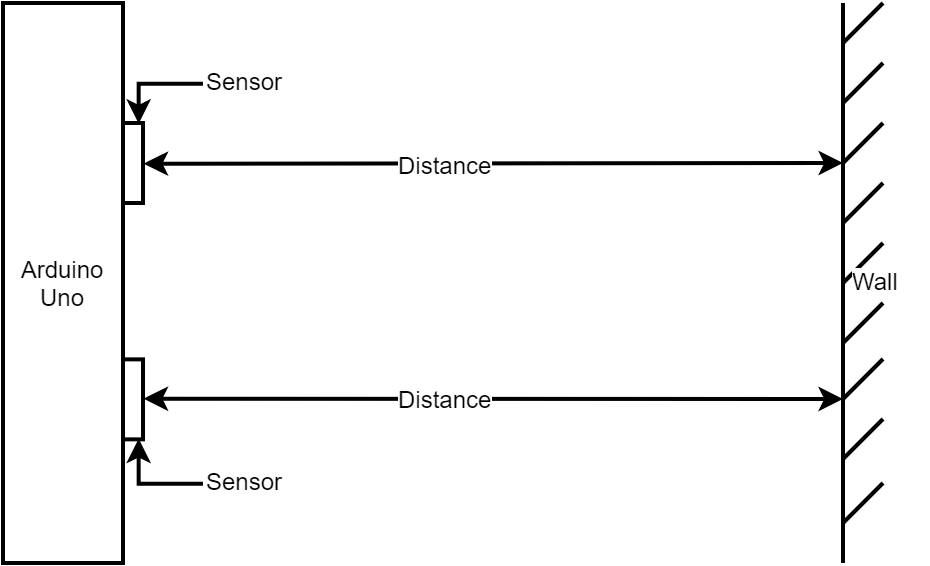
\includegraphics[width=0.6\textwidth]{figures/Appendix/testopstillingSensor.png}
    \caption{Illustration of the test setup.}
    \label{fig:testSetupSensor}
\end{figure}

%
\section*{Execution}
The code used to test the sensors can be found in the github repository \url{https://github.com/AAU-EIT5/VL53L0X-sensor-test}. The code is getting a 100 readings from the sensor, and then printing them out in the arduino monitor.
\newline
The first test are executed by taking readings with the sensors from different distances, starting from 30 cm and ending at 110 cm, with a interval of 10 cm between each. The distances a measures with a measuring tape.
\newline
The second test are executed at a distance of 110 cm, where the sensor broad is with the angel +10$\degree$ and -10$\degree$. 

%
\section*{Results}
For the first test can the results for sensor 1 can be seen on figure \ref{fig:resultatSensor1test} and for sensor 2 in figure \ref{fig:resultatSensor2test}. The average time the sensors took to measure a 100 values at adjusted time of 20 ms is 1848961 microseconds, which approximately equals to 18.5 milliseconds, that gives a sampling rate of 54 Hz. 

\begin{figure}[H]
    \centering
    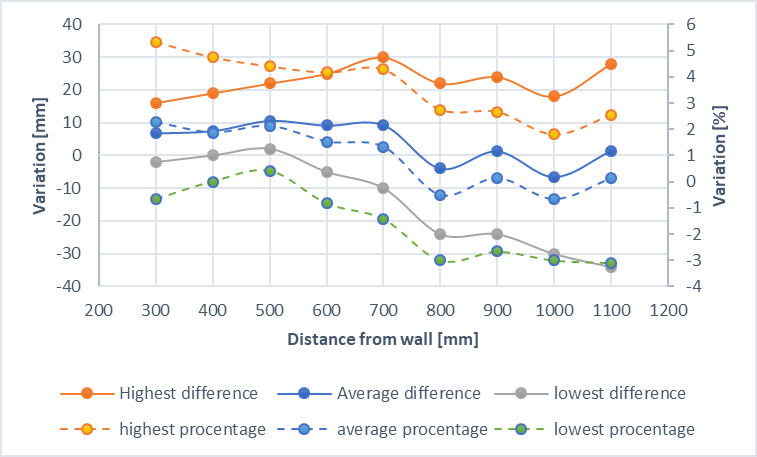
\includegraphics[width=0.8\textwidth]{figures/Appendix/resultatSensor1Test.png}
    \caption{Results from sensor 1.}
    \label{fig:resultatSensor1test}
\end{figure}
\begin{figure}[H]
    \centering
    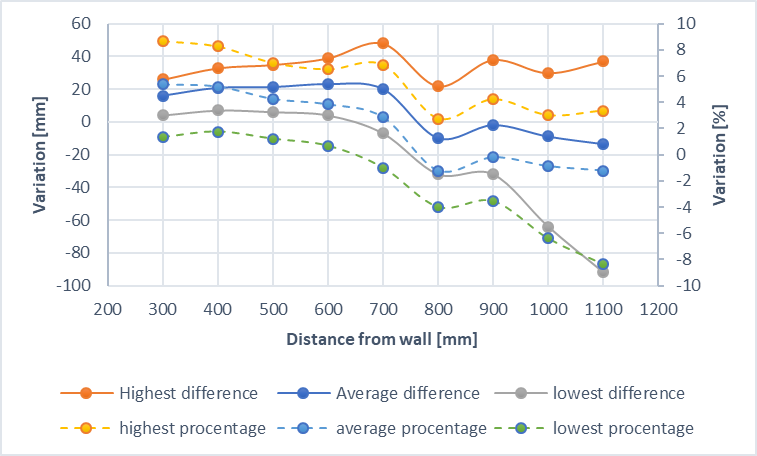
\includegraphics[width=0.8\textwidth]{figures/Appendix/resultatSensor2Test.png}
    \caption{Results from sensor 2.}
    \label{fig:resultatSensor2test}
\end{figure}

The results from the test to see if the sensors could detect a wall when it have a angel of $\pm 10 \degree$ can be seen in table \ref{tab:sensorAngelRes}.
\begin{table}[H]
    \centering
    \caption{Results from test of sensors with a angle of $\pm 10 \degree$.}
    \label{tab:sensorAngelRes}
    \begin{tabular}{|c|c|c|}
    \hline
             & \textbf{10$\degree$ left} & \textbf{10$\degree$ Right}  \\ \hline
    \textbf{Results sensor 1:} & Detected in all readings  & Detected in all readings    \\ \hline
    \textbf{Results sensor 2:} & Detected in all readings  & Detected in all readings    \\ \hline
    \end{tabular}
\end{table}

%
\section*{Discussion}
From figure \ref{fig:resultatSensor1test} and \ref{fig:resultatSensor2test} can it be seen that the sensors can detect a wall that are at lest op to 1100 mm. As one of the requirements the sensors have to hold are a detection of a wall at minimum 1000 mm, do the sensors comply with this requirement.
\newline
\newline
Another requirement the sensor have to comply is a accuracy of $\pm 10 \degree$ at 400 mm distance from a wall. If figure \ref{fig:resultatSensor1test} can there be notice a variation of around 0 $\%$ to around 5 $\%$ from the actual distance and as the requirement for the sensors is $\pm 5 \%$, sensor 1 comply with it. On the other hand, do sensor 2 not comply with the requirements, as it's variation a 400 mm is from around 1 $\%$ to around 9 $\%$, but as it can be observed from the figures \ref{fig:resultatSensor1test} and \ref{fig:resultatSensor2test}, are the averages measurements both shifted from the actually distance from the wall. If the shifted distance are taking into account, are the accuracy of both sensors with ind the required accuracy. 
\newline
\newline
Some of the factors that can cause the shifting of the distance, is firstly the measured distance with measuring tape the sensors where placed can be inaccurate with a few millimeters. secondly the board the sensors where on could have a slight angle, there one sensor then would be closer to the wall than the other. lastly the sensors measuring can be off, when initializing the sensors.
\newline
\newline
The third requirement the sensors have to abide are a sampling rate of a 40 Hz, and as the measured sampling rate of the sensors are 54 Hz, meets the sensors the requirement. As the sensors where set to a sampling rate of 50 Hz, can the difference of 4 Hz be because of the sensors where faster to get a reading than enlightened from the datasheet.
\newline
\newline
Lastly a requirement for how high a angel the sensors have to detect the wall was set $\pm 10 \degree$, where both sensors could detect them a 1100 mm distance. Some of the uncertain factors for this test, are the precise angle of the board, as it could variate a couple of degrees. The exact distant could also vary a couple of mm, but as the measured distance to the wall was lager than 1 meter this have no influence of the results.

%
\section*{Conclusion}
From the results of the test, can there be concluded whether the sensors comply with the requirements. the first requirements the sensor have to comply with are the detection of a wall of 1 meter, and as it can detect the wall a 1.1 meter distance it meets with the requirement.
\newline
The second requirement the sensor have to comply are a accuracy of $\pm 5 \%$ at 400 millimeters, that it only meets of the shifted distance of the sensors, where it then have a a accuracy of op to $\pm 4 \%$.
\newline
The third requirement the sensors have to meet are a sampling rate of 40 Hz, that it meets as it can have a sampling rate op to 54 Hz.
The last requirement the sensor have to meet are the angle of $\pm 10 \degree$ which the sensors have to detect, and from the test it can be seen that i sensors can detect the wall at this distance.
\newline 
Over all are all the requirements meet with the sensors, if the shifting of the distance are taking into account. 